\documentclass[a4paper,3p,sort&compress]{elsarticle}

\usepackage[draft]{hyperref}
\usepackage{url}
\usepackage{booktabs}
\usepackage{graphicx}
\usepackage{xspace} 
\usepackage{booktabs}
\usepackage{makecell}
\usepackage{lineno}
\usepackage{natbib}
\usepackage{amsmath}
\DeclareRobustCommand{\citeext}[1]{\citeauthor{#1}~\cite{#1}}

\usepackage[nomargin,inline,draft]{fixme}
\fxsetup{theme=color,mode=multiuser}
\FXRegisterAuthor{j}{jla}{\color{purple}JLA}
\FXRegisterAuthor{s}{spv}{\color{teal}SPV}
 
\journal{-}

%% `Elsevier LaTeX' style
\bibliographystyle{plain}
%%%%%%%%%%%%%%%%%%%%%%%

\begin{document}
\linenumbers

% Macro para escribir NO$_2$
\newcommand{\no}{NO\textsubscript{2}\xspace}

\begin{frontmatter}

  \title{Introducing a novel visualization technique for time series uncertainty visualization}


  \author{Sebasti\'an P\'erez Vasseur}
  \author{Jos\'e L. Aznarte}
  \address{Artificial Intelligence Department\\Universidad Nacional de
    Educaci\'on a Distancia --- UNED\\c/ Juan del Rosal, 16, Madrid, Spain}
  \ead{jlaznarte@dia.uned.es}
  

\begin{abstract}
  
\end{abstract}

\begin{keyword}
probabilistic forecasting \sep visualization \sep natural frequency chart
\end{keyword}

\end{frontmatter}

%\linenumbers

\section{Introduction}
\label{sec:intro}

From the early stages of data processing and decision making, analysts are confronted with uncertainty. This uncertainty
has several sources: incomplete information, missing values, unpredictability of the future ... As stated by Padilla et al.,
taking it into account is essential to estimate the potential risks and rewards derived from the decisions. 

For example in the context of weather forecast, Joslyn et al explain 
that people can use uncertainty to correct invalid biases from their expectations (whih bias and exectatinos ?).
Also in weather forecast, Rouston et al. 
\cite{roulston_laboratory_2006} showed that analysts could improve their rewards and reduce their exposure 
to risk how ? Elaborate. 

One of the primary examples of this is when basing our decisions on machine learning forecasts.
One way to present uncertainty is to present probabilistic forecasting, which instead of showing the evolution 
of the predicted value of a target variable, presents the evolution of the full distribution or main quantiles 
of the target variable. Pinson et al. mentions how the presence of the uncertainty permits to optimize the value 
of wind energy generation. In air quality forecasting, Perez-Vasseur et al. showed how probabilistic forecasting 
enables the estimation of the probability the No2 pollutant will reach a certain threshold and become a danger 
to the city inhabitants.

However, uncertainty visualization and understanding has faced many challenges. As Padilla et al. \cite{balakrishnan_uncertainty_2021} 
points out, this could be due not only to the abstract nature of probability 
but also to poor communication techniques. Weiskopf et al. reaches a similar conclusion and states 
that uncertainty understanding should be linked to the way it is communicated. 

One area of research which could alleviate this problem is data visualization. Indeed, as 
stated by Islam et al., visualizations are easier for the human brain to understand and process.
For instance, Perez Cota et al. mentions how visualization are playing an important role in the business 
environment where all the analytical tools are embracing visualization to better understand large quantities of data. 

\section{State of the art}
\label{sec:results}

One of the most typical approaches, Visual Boundaries such as isocontours and error 
bars display value areas within a certain confidence interval. The problem with this approach is 
that individuals may exclude as possible values outside the confidence interval, which are still 
possible, only less probable. 

Also, Belia et al \cite{belia_researchers_2005} showed that even leading researchers had 
trouble reading error bars and they confused 
standard errors and confidence intervals. 

In addition, Joslyn and LeClerc showed that individuals could also be inclined to take uncertain 
information as deterministic, for example by considering the confidence interval for whether temperature 
forecast as high and low temperature. 

As noted by Joslyn et al. \cite{joslyn_communicating_2010}, this has lead to a new surge of 
research in visualization techniques: Van 
der Bles et al. \cite{van_der_bles_communicating_nodate} point that there is more than 
error bars to show uncertainty. 

One possible solution to this problem is the use of HOPs (hypothetical outcome plot). HOPs display 
sequentially in an animation, random values from a distribution. However, this technique can not be 
applied to static visualizations. 

An alternative approach, Visual Semiotics uses visual encoding such as fuzziness or color to represent 
the probability of a certain value. An example of this would be the use of gradients to represent the 
full probabiliity distribution. Neverthless, this type of encoding makes it difficult to read specific 
values. Finally, Frequency Framing uses natural frequencies to display probabilities. As noted by Gerd 
Gigerenzer, individuals prefer frequencies or ratio, like 1/10, when understanding probability. This has 
lead to the development of the quantile dot plot. This plot, created by Kay et al. 
\cite{2016-when-ish-is-my-bus} 
represents 
the probability distribution with dots: by using 20 dots, each would represent 1/20 probability 
and are placed according 
to the quantiles of the distribution. Quantile dot plot have proved to lead to better distribution 
understanding and probability estimates reading. 

However those approaches do not address specifically the problem of uncertainty in the case of time series.
The visualizations would need to show the evolution of uncertainty in time: this 
is especially challenging as a visualization must display several distributions in a constrained space.  
As pointed out by Leffrang et al. \cite{leffrang_should_2021}, not much research has been applied to the 
field of uncertainty visualization in this field. 
However, we have already seen in the literature solutions for this problem as confidence interval charts,
 box plots or gradient charts. Those 3 types of charts correspond to the different solutions for uncertainty 
 we have seen above. However, we have not seen yet a solution involving frequency framing. As stated by van Wijk,
 data visualization can be considered an art and therefore subject to criteria like taste or design aesthetics. 
However, we can also evaluate the performance of those visualizations on probability readability.
Brenner et al. \cite{brennen_instrument_2018} developed a methodology to systematically evaluate the performance
of uncertainty visualizations, based on four measures: cognitive load, confidence, accuracy and time to read. 

Therefore, inspired by Brenner et al., we propose a social experiment where we will compare those charts 
in terms of probability reading: confidence interval, time series box plot, visual semiotics.
Also, we are introducing a novel type of chart based on frequency framing: Natural frequency time chart.

We will use as an application ground for this comparison a probabilistic forecast of NO levels 
in the city of Madrid. This forecast contains the full predicted distribution of NO levels over time
and we display this very same time series with uncertainty in each of the visualization mentioned above. 
We then estimate for each one how well its numeric values are read by assessing how several individuals read 
and understand the charts.

\section{Time Series probabilistic charts}  
\label{sec:time_series}

Figure \ref{figure:charts} shows a summary of the studied probabilistic time series charts.

The confidence interval chart shows in a line the evolution of the median of the distribution
 over time alongside 2 lines: the evolution of the 5\% and 95\% percentile of the distribution. 
 User estimates the probabilities with the distance of the points to those lines.

The box plot chart shows different percentile with “boxes”. For each point in time, a white 
line shows the location of mean, then a rectangle (or box) lower and upper part is located 
at the 25\% and 75\% percentile respectively, a narrower box upper and lower part shows 
the 5\% and 95\% percentile and finally a line’s edge shows the 1\% and 99\% percentile. 
This visual boundary representation shows more percentile than the confidence interval and 
is recommended when the distribution is not symmetrical and to show the edges of the distribution.

The gradient chart shows the evolution of the median in a line and then displays the different percentiles
with overlapping areas whose color corresponds to the percentile. We end up having an area with a gradient 
delimited by 2 lines: the 1\% and 99\% percentile. This representation allows to have the
 full range of percentiles represented.

The 3 methods described above have been used in the literature as a way to display the overall uncertainty 
of the target variable. However, they are not designed for probability readability: for example, to determine 
the probability the target variable is within a certain range or above a certain value. Also,
each of the methods have their own shortcomings. The confidence interval gives a false sense of determinism as mentioned previously
and values outside of the interval will not be taken into account. The confidence interval is also not a good solution 
when the distribution of the target variable has a long tail. The box plot shows only some percentiles and it can be difficult to 
estimate the probabilities from the boxes boundaries. Finally, although the gradient displays the most information, it has been 
proven that color is not 
a good visual encoding and is more difficult to read than other encodings. We plan on showing those shortcomings during the comparison in our experiments.

Since no solution was based on natural frequencies, we decided to apply the idea for time series and design the natural frequency time chart.
This visualization is a novel technique based on frequency framing and has 
specifically been designed for probability readability. First, 
it shows the evolution of the median of the distribution in a line. And then, for each time 
step, 10 percentiles from 5\% to 95\% (5\%, 10\%, 15\%, ...) are represented: this way, we can estimate the percentage 
probability of being in an interval as 10 times the number of circles in that interval. 
We have chosen 10 percentiles as it makes it easy to calculate the probability (just multiply by 10), also a higher number
would have cramped the chart and made it difficult to view the circles as separate. 


\begin{figure}
  \centering
  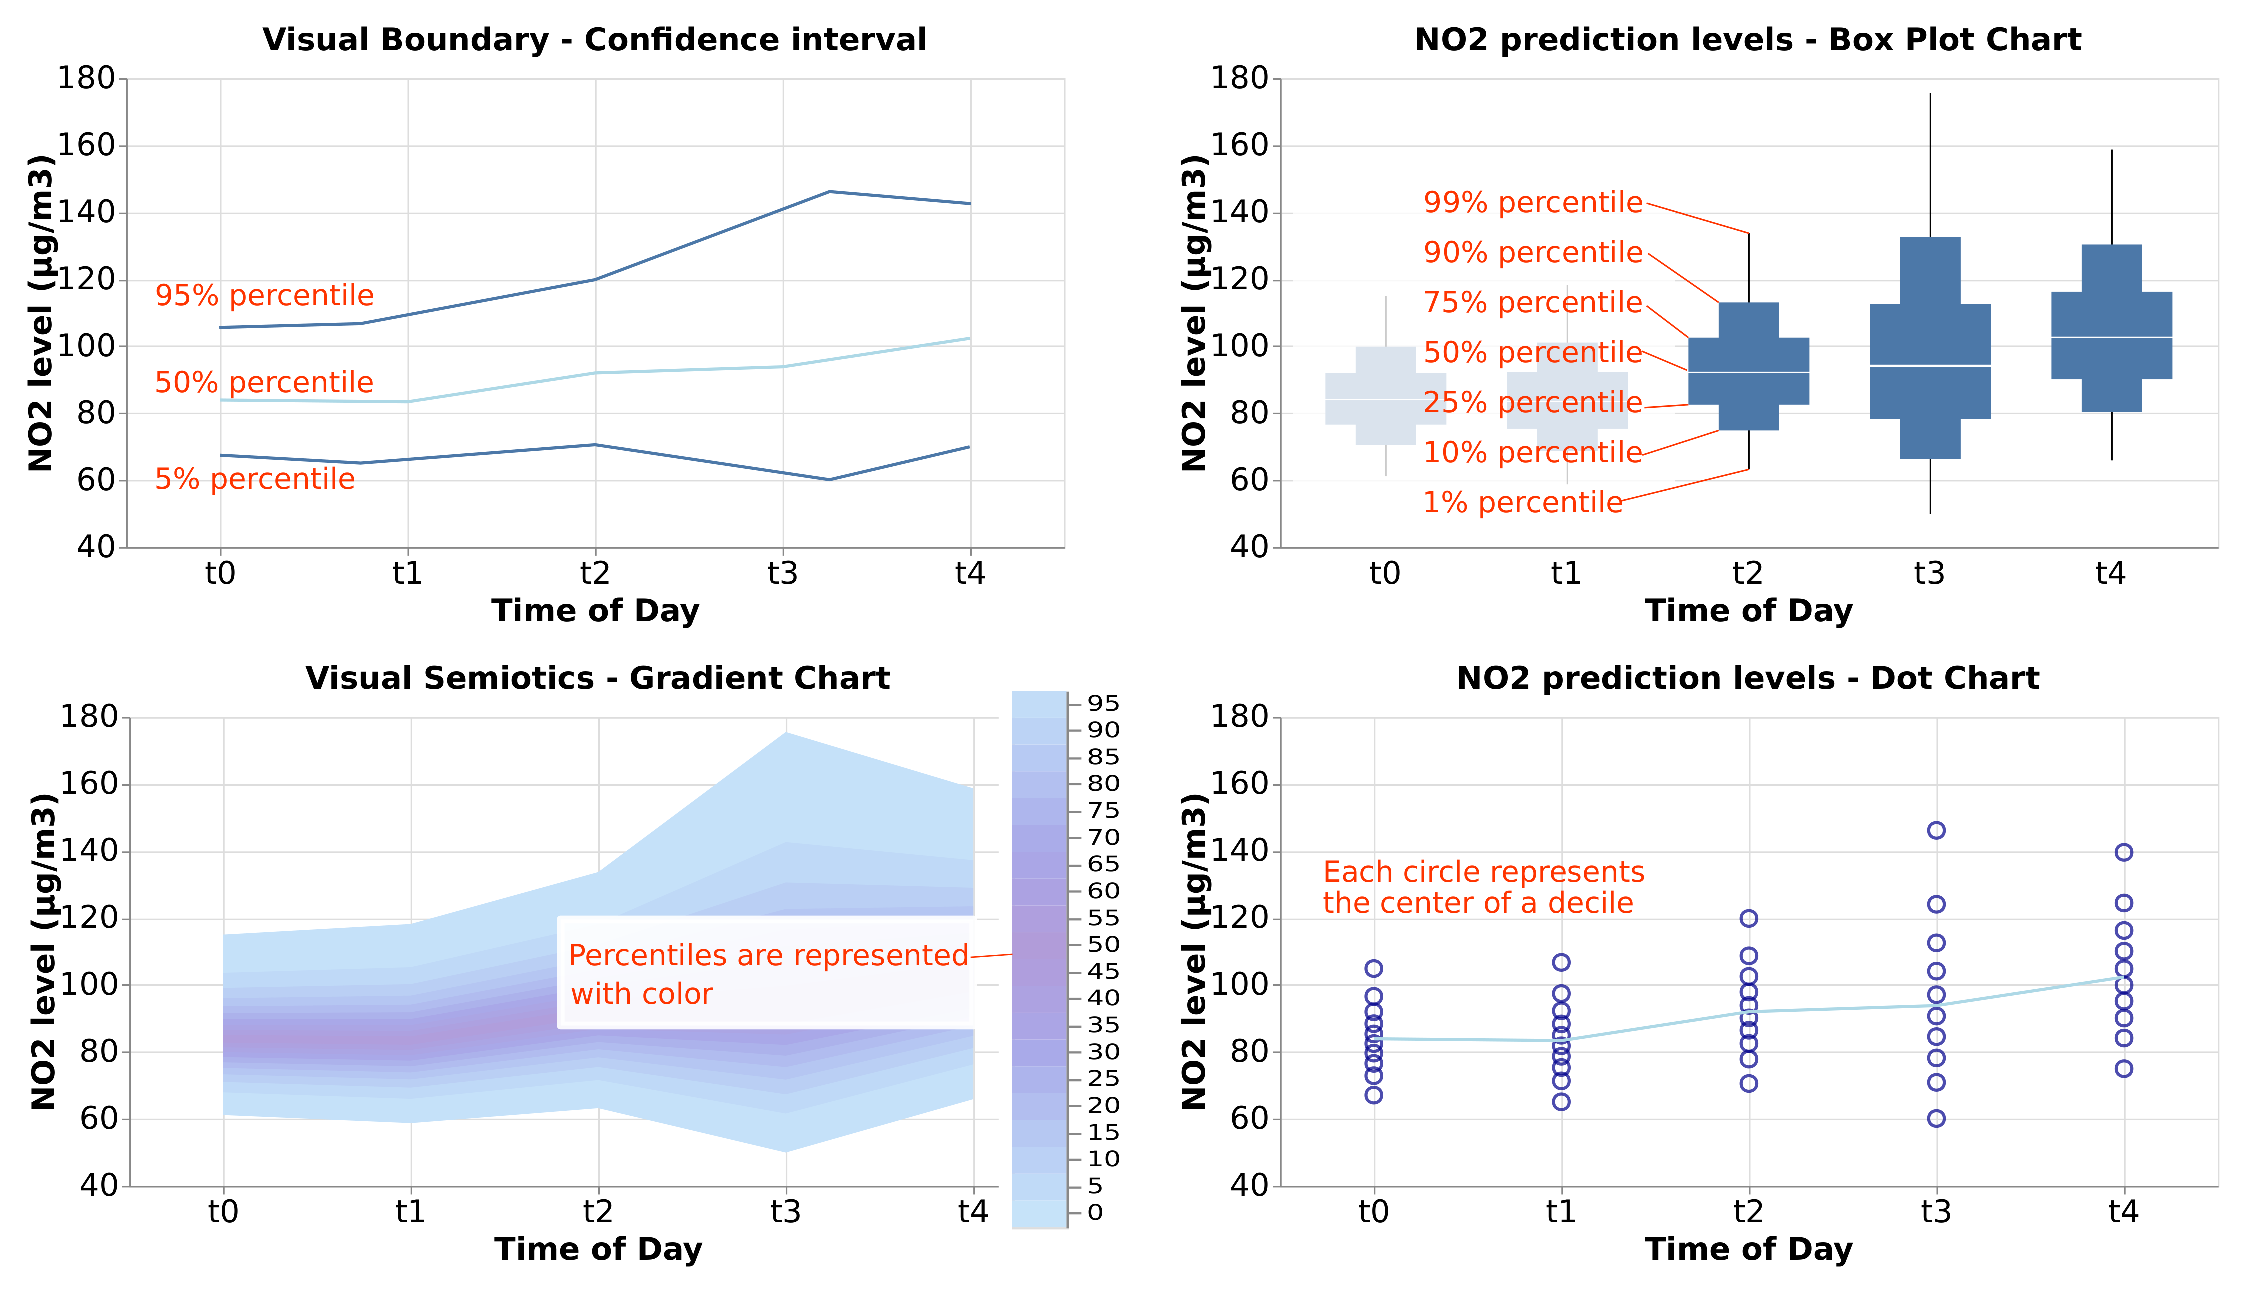
\includegraphics[width=.9\textwidth]{charts_vector} 
  \caption{\label{figure:charts} Probabilistic Forecast of NO2 levels in Madrid with different types of time Series Chart. 
  Top Left: Confidence Interval. Top Right: Box Plot. 
  Bottom Left: Gradient Chart. Bottom Right: Natural Frequency Time Chart. }
\end{figure} 

\section{Experimental Design}
\label{sec:exp_design}

We compare the readability of the four main types of probabilistic time series charts 
displayed in figure 1. We evaluate how well the charts can be read to estimate the probability 
that the evolving target is within a certain interval at a certain time point. As stated previously, 
the evolving distribution is the probabilistic forecast of NO levels. 

For this, we request the participation of users through the Amazon Mechanical Turk website. 
This service picks randomly 100 individuals with a minimum skill set (as proposed by Brenner 
et al. \cite{brennen_instrument_2018}, we select Master level participants, who are workers who 
''have consistently demonstrated a high degree of success in performing a wide range of HITs across a 
large number of Requesters'').

Each individual is presented a unique type of chart from the 4 presented above, gets a brief 
explanation on how it works and they have to estimate 5 probabilities from the chart. An example question is: 
"What is the probability of the NO2 levels being between 150 and 200 on 
November 21st at 22:00 ?". We are also measuring the time it took to perform each estimation. 
As inspired by the work of Brenner et 
al. , once the individuals have estimated the probabilities, they are asked how confident they 
felt and how difficult the task was considered.

We are testing 20 individuals per type of chart and therefore we have 100 answers per 
type of chart.

\section{Results}
\label{sec:results}

First, for each answer, we define the 
reading error as the absolute value of the difference 
between the provided answer and the true probability displayed in the chart. Figure \ref{figure:errors} shows 
the distribution of the reading error per type of chart. We see clearly how the natural frequency time chart
has a much lower reading error then the other charts. 

\begin{figure}
  \centering
  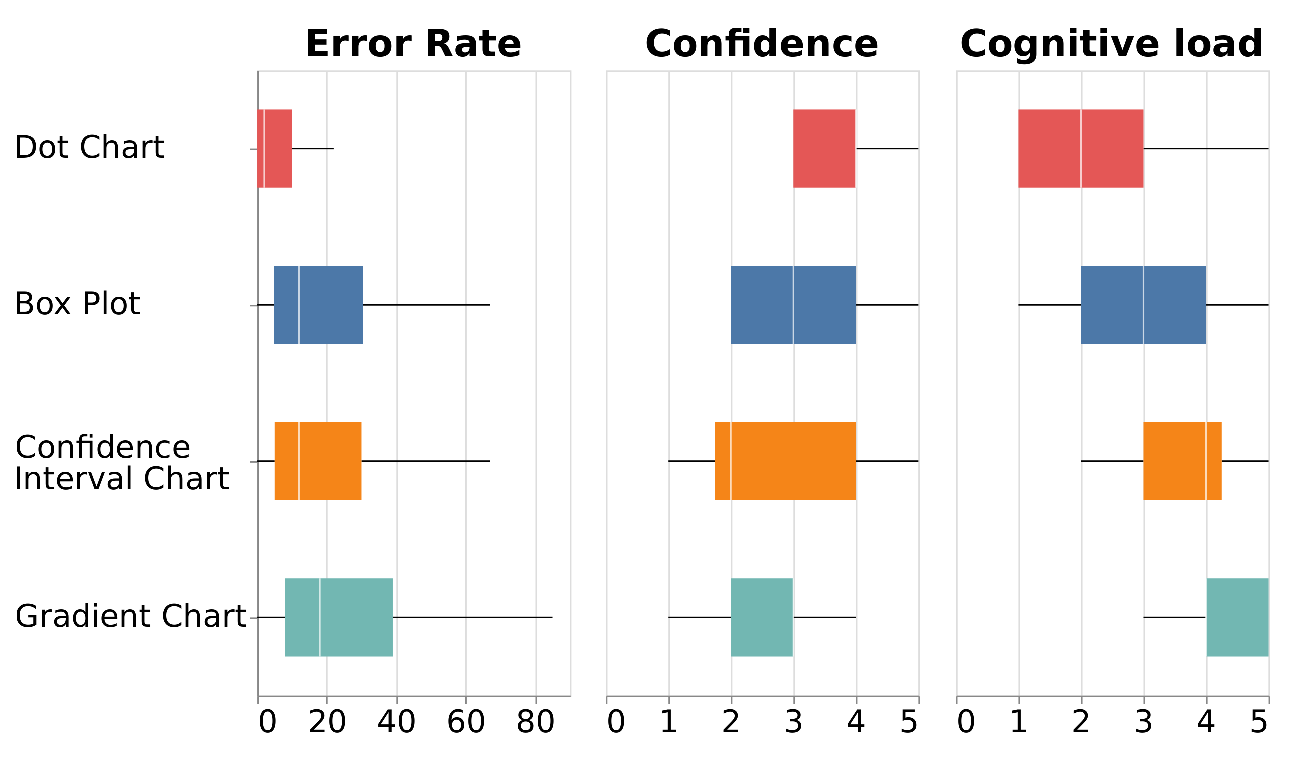
\includegraphics[width=0.8\textwidth]{comparison}
  \caption{\label{figure:errors}Reading Error, confidence and perceived difficulty per 
  type of visualization. Black vertical line represents median.
  The whiskers represent the 10 and 90 percentile and the box shows the 25 and 
  75 percentile.}
\end{figure}


\begin{table}[h!]
  \centering
  \begin{tabular}{lrr}
    \toprule
    {}Question &     Error Mean &        Error Std Deviation \\
    \midrule
    1 &  19.4 &  16.8 \\
    2 &  20.7 &  12.1 \\
    3 &  10.9 &  18.9 \\
    4 &  27.0 &  26.9 \\
    5 &  16.1 &  15.6 \\
    \bottomrule
    \end{tabular}
  \caption{Error}
  \label{table:resultsperquestion}
  \end{table}

We see in figure \ref{figure:duration} that for every chart, the time it takes 
to read and answer the question decreases for every question answered. As we see in the figure, those times 
are very similar for all the types of charts. 

\begin{figure}
  \centering
   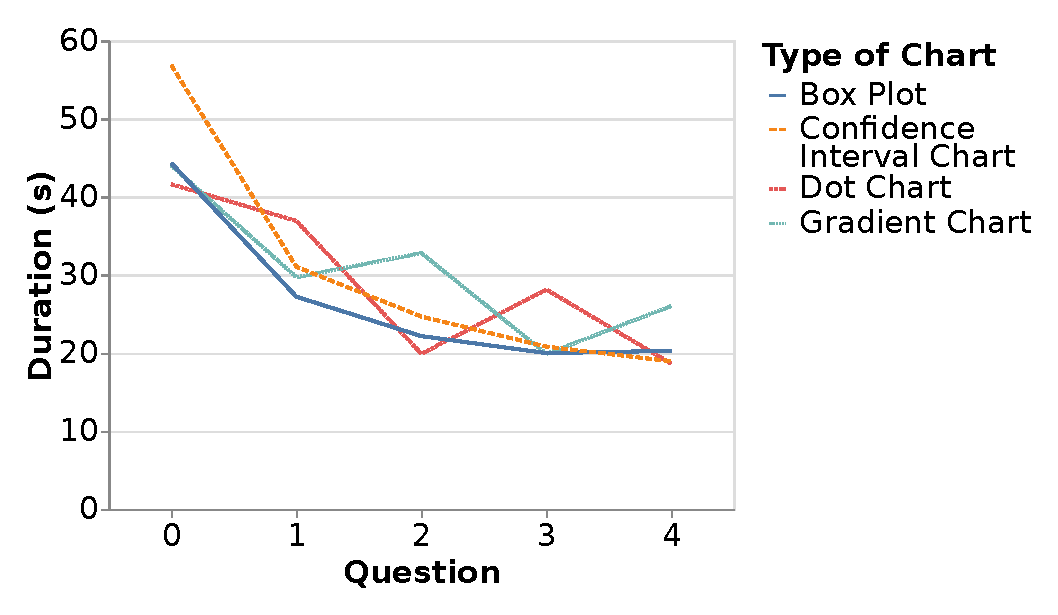
\includegraphics[width=0.6\textwidth]{duration_evo2}
  \caption{\label{figure:duration} Median Time it took to answer each question for each of the types of chart.}
\end{figure}  

Confidence and perceived difficulty charts (also shown on figure \ref{figure:errors}) also show the superior ease of use 
of the natural frequency time chart. Users reported higher levels of confidence and 
lower levels of perceived difficulty for the natural frequency time chart.

Finally although we selected users with master level, we still did received answers with probabilities 
above 1 or a probability as an interval. This could be due a lack of statistical knowledge from those 
users and reinforces the fears discussed in the introduction. 
We identified 9 users from 80 whose answers could not be used because of those reasons.

\section{Conclusions}
\label{sec:concl}

Although we could remark that the gradient chart, the box plot or the confidence interval charts are very good at 
providing an overall picture of the uncertainty in the time series, we can see from this work that the application of natural 
frequencies in an uncertainty chart does indeed
provide better numeric readability than any previous alternative. Natural frequencies does indeed simplify 
the statistic knowledge requirement and is also easier to read as it consists on counting.
We could improve even more the ease of use with interactive elements in the chart: for example
by applying different colors to the circles within a certain interval defined by the user interactively.

This type of chart is less well known that the other alternatives and an information effort should be made to motivate 
researchers and the general public to use it.

\section{References}
\label{sec:ref}


\bibliography{refs}

\end{document} 

